\section{Introduction}
%%%%%%%%%
% 引入,通过从其他任务或者现实情况中,
%%%%%%%%%
When solving a problem, it is crucial to develop a plan or determine a specific sequence. Procedure planning particularly addresses issues related to planning and sequencing. It is an essential and fundamental reasoning ability for tackling real-world challenges such as robotic navigation \citep{sermanet2024robovqa,bhaskara2024trajectory} and autonomous driving \citep{wang2024driving,liao2024bat}. In this context, identifying the actions involved and determining their temporal and causal relationships enables the model to reason and infer logically based on the current conditions.
%%%%%%%%%%%

% 简要概括前人工作的重点,最后说明仍然存在的问题
%%%%%%%%%%
Initially, we must consider where the temporal and logical relationships of actions are embedded. For instance, in the task of cooking~\citep{bollini2013interpreting}, the ``preparing ingredients'' should precede ``cooking''. The model should recognize that the action of ``cooking'' is a subsequent step that relies on prior events; similarly, there should be an awareness of the logical sequence between ``washing vegetables'' and ``cooking a meal''. This principle applies equally to various other reasoning tasks. Recent studies have primarily utilized weakly supervised methods \citep{zhao2022p3iv}, the simple application of diffusion models \citep{wang2023pdpp}, specific strategies to aid model judgments \citep{nagasinghe2024not,wang2023event}, or a focus on state changes \citep{niu2024schema}. Up to now, to the best of our knowledge, few papers have considered learning the temporal and logical relationships between actions.
% In contrast, our approach places a greater emphasis on learning the temporal and logical relationships between actions.

%%%%%%%%%%%
% 说明本文主要的目的和改进点,通过引用一些跟我的创新点相关的paper,引出我想要做的东西
%%%%%%%%%%%%
This paper aims to establish a more robust temporal and logical structure to capture the causal logic sequence between actions. But what exactly is a causal logic sequence in the context of procedure planning? \citet{gruver2024large} frames time series forecasting as next-token prediction in text by encoding time series as a string of numerical digits. \citet{xiong2024teilp} establishes a logical reasoning framework that naturally integrates temporal elements into knowledge graph predictions. 
LDM~\citep{rombach2022high} and VideoLDM~\citep{blattmann2023align} transfer the original data into latent space. The success of transforming action relationships into other structures or just using latent motivates us to investigate the latent features hidden within the action sequence.

%%%%%%%%%%%
% 介绍我的工作是什么,核心是什么,为什么这么做,具体解释。
%%%%%%%%%%%%
In this work, we achieve this goad by fusing an interpolation predictor into masked diffusion.  The cores of our method are temporal logic modeling of potential features. For temporal logic modeling, motivated by success of StoryDiffusion~\citep{zhou2024storydiffusion} in long video generation and VideoLDM~\citep{blattmann2023align} with latent processing, we construct a temporal interpolation predictor to capture logic relationship between actions and process them in the state of latent. Then we apply simple linear interpolation to latent for completing the remaining components by using given start and end visual features. Subsequently, we use cross-attention to input the potential features filled by interpolation into the iterations of the original diffusion model to assist in generation. To limit the scope of action generation, we also add masking mechanisms in the generation and loss penalty of diffusion models. Finally, the temporal interpolation predictor is trained in the masked scopes.

% \begin{figure}[h]
% \begin{center}
% %\framebox[4.0in]{$\;$}
% \fbox{\rule[-.5cm]{0cm}{4cm} \rule[-.5cm]{4cm}{0cm}}
% \end{center}
% \caption{Sample figure caption.}
% \end{figure}
\begin{figure}[t]
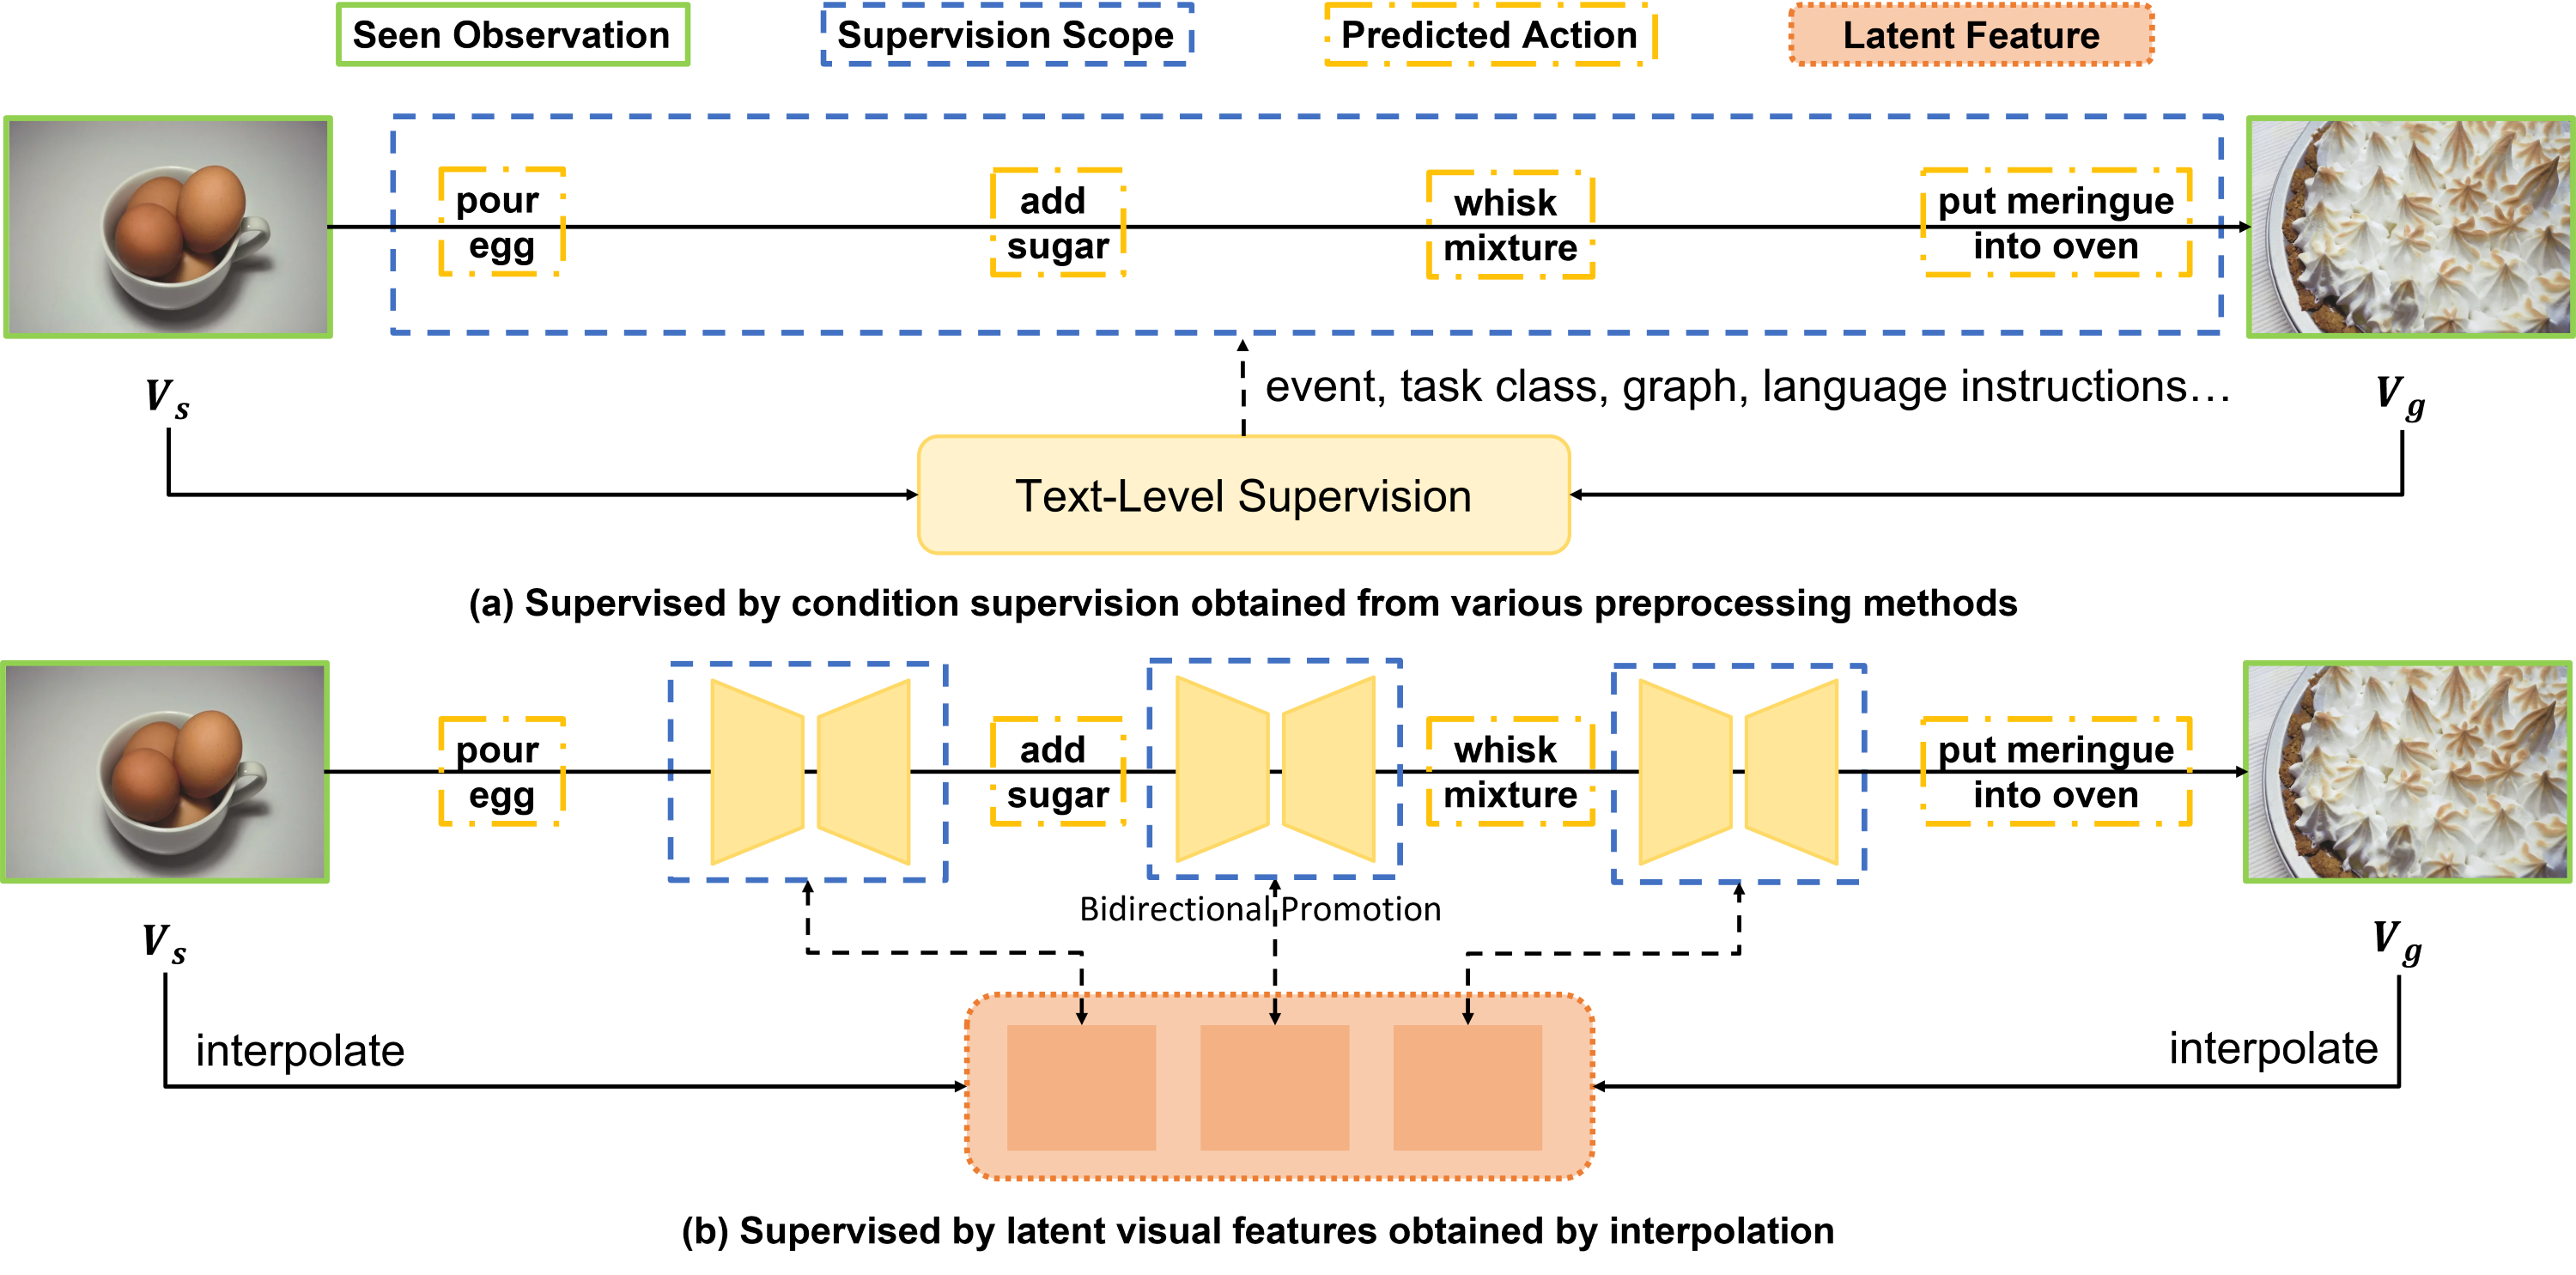
\includegraphics[width=0.98\textwidth, keepaspectratio]{figures/fig-task.png}
% \vspace{-0.5em}
\caption{The core idea to solve procedure planning with previous methods and ours. }
\label{fig:task}
% \vspace{-2.5mm}
\end{figure}
%%%%%%%%%%%%%%
% 总结我们的主要贡献
%%%%%%%%%%%
The main contributions of this paper are as follows:
\begin{enumerate}
 \item \textbf{A masked temporal interpolation predictor:} While inheriting the basic model of PDPP, this predictor absorbed the experience of StoryDiffusion and innovatively used masks to limit the range of actions, thus improving the accuracy of generated actions.
 \item \textbf{Using interpolated predictors and latent feature extraction methods:} The model generation was enhanced by inputting start and end frames, extracting potential features using encoder, and generating latent features for intermediate frames through interpolation strategy to further guide the intermediate process of diffusion model.
 \item \textbf{Experimental validation was performed on different types of datasets:} In this paper, we conducted extensive experimental validation on CrossTask, COIN, and NIV datasets, and the results showed that the method proposed in this paper significantly improved the model performance on several tasks.
\end{enumerate}
